% 
% Annual CCN conference
% Sample LaTeX Two-Page Summary -- Proceedings Format
% based on the prior cognitive science style file

% Original : Ashwin Ram (ashwin@cc.gatech.edu)       04/01/1994
% Modified : Johanna Moore (jmoore@cs.pitt.edu)      03/17/1995
% Modified : David Noelle (noelle@ucsd.edu)          03/15/1996
% Modified : Pat Langley (langley@cs.stanford.edu)   01/26/1997
% Latex2e corrections by Ramin Charles Nakisa        01/28/1997 
% Modified : Tina Eliassi-Rad (eliassi@cs.wisc.edu)  01/31/1998
% Modified : Trisha Yannuzzi (trisha@ircs.upenn.edu) 12/28/1999 (in process)
% Modified : Mary Ellen Foster (M.E.Foster@ed.ac.uk) 12/11/2000
% Modified : Ken Forbus                              01/23/2004
% Modified : Eli M. Silk (esilk@pitt.edu)            05/24/2005
% Modified : Niels Taatgen (taatgen@cmu.edu)        10/24/2006
% Modified : David Noelle (dnoelle@ucmerced.edu)     11/19/2014
% Modified : Konrad Kording (koerding@gmail.com) 2/15/2017

%% Change "letterpaper" in the following line to "a4paper" if you must. 
% Alternatively, just ignore that because who prints papers anymore?

\documentclass[10pt,letterpaper]{article}


\usepackage[utf8]{inputenc} % allow utf-8 input
\usepackage[T1]{fontenc}    % use 8-bit T1 fonts
\usepackage{hyperref}       % hyperlinks
\usepackage{url}            % simple URL typesetting
\usepackage{booktabs}       % professional-quality tables
\usepackage{amsfonts}       % blackboard math symbols
\usepackage{nicefrac}       % compact symbols for 1/2, etc.
\usepackage{microtype}      % microtypography

\usepackage{amsmath}
\usepackage{graphicx}
\usepackage{ amssymb }
\usepackage{mathtools}
\usepackage{algorithm}% http://ctan.org/pkg/algorithms
\usepackage{algpseudocode}% http://ctan.org/pkg/algorithmicx
\usepackage{setspace}
\usepackage{xcolor}
\usepackage{makecell}
\usepackage{ccn}
\usepackage{pslatex}
\usepackage{apacite}

\title{Fast Weights Using Improved Memory Consolidation Designs}
 
\author{{\large \bf Bowen Xu (bowenxu@cs.toronto.edu)} \\
  Department of Computer Science, University of Toronto \\
  10 King's College Road, Rm. 3302, Toronto, Ontario, Canada, M5S 3G4
  \AND {\large \bf Jimmy Ba (jimmy@psi.toronto.edu)} \\
  Department of Electrical \& Computer Engineering, University of Toronto \\ 
  10 King's College Road, Rm. 3302, Toronto, Ontario, Canada, M5S 3G4
  \AND {\large \bf Richard Zemel (zemel@cs.toronto.edu)} \\
  Department of Computer Science, University of Toronto \\
  10 King's College Road, Rm. 3302, Toronto, Ontario, Canada, M5S 3G4}


\begin{document}

\maketitle


\section{Abstract}
{
\bf
Storing better quality and greater amount of memory has been a difficult challenge for deep learning.
While the current artificial neural networks excel at tasks such as regression and classification, they fail to perform equally well on representing variables and storing data over long time.
In this paper, we introduce an enhanced fast weights model that includes robust memory consolidation designs into the existing memory transformation mechanisms.
We show that our model comes with no additional costs, converges faster, and out-performs the original fast weights model on the associative retrieval tasks.
}
\begin{quote}
\small
\textbf{Keywords:} 
Fast Weights; Memory Consolidation; Memory Transformation; Deep Learning; Associative Retrieval
\end{quote}

\section{Introduction}
Retaining more memory for a longer period of time is an important goal for any memory system.
Recently, Benna and Fusi have demonstrated that the combination of a power-law memory decay with a fast new memory adaptability maximizes both the memory storage and lifetime (2016).
Their method treats each piece of memory as random and uncorrelated, and maximizes the signal to noise ratio (SNR) of all the stored memories \cite{pld}.
%Recent advances in artificial neural networks \cite{dnc, fw} have illustrated different ways of combining the external memory with the artificial neural networks.
%However, their models are either designed with over-complicated memory management systems \cite{dnc} or not designed to protect against memory interference and overwriting \cite{fw}.

We adopt and adapt some of Benna and Fusi's ideas to current deep learning systems, notably the fast weights work \cite{fw}.
%We devise a robust Fast Weights model that adopts better memory consolidation designs. 
%Our external memory fully incorporates the most recent memory change while decaying the previous memory storage following a power-law decay.
%The memory consolidation designs are proved to reduce memory overwriting and interference problems.
We show that our approach leads to a faster convergence and  a stronger testing accuracy for the fast weights model on the associative retrieval tasks.


\section{Background}
%\subsection{Fast to Slow Memory Transformation}
Recent advances in deep learning \cite{dnc, fw} have shown that the use of an external memory with the artificial neural networks can significantly improve their abilities to retain information.
%Ba et.\ al.\ devise a bidirectional memory transformation system that improves neural networks' ability to retain information for longer \cite{fw}.
Ba et.\ al.\ devise a bidirectional memory transformation system.
Knowledge is not only transferred from the fast weights to the memory cells of a Recurrent Neural Network (RNN) through its hidden vector update but also transitioned from the memory cells to the fast weights as it is updated using the latest hidden vector at each time step.
Also, a learning rate $\eta$ and a decay rate $\lambda$ are included to control how much the fast weights should store new knowledge versus how quickly it should forget previous knowledge.
\begin{align}
    &A(t) = \lambda A(t-1) + \eta h(t) h(t)^T
    \label{eq:external_memory} \\
    &h_s(t+1) = f(LN(Wh(t) + Cx(t) + A(t)h_{s-1}(t+1)))
    \label{eq:hidden_update} \\
    &h(t+1) = h_s(t+1) \label{eq:hidden_assign} \\
    &w_a(t) \equiv \sum_{t^{'} < t} \Delta w_a(t') r(t-t')
    \label{eq:memory} \\
    &S_{t^{'}}(t) \equiv \frac{1}{N}\left<\sum_{a=1}^N w_a(t)\Delta w_a(t') \right>
    \label{eq:signal} \\
    &N^2_{t^{'}}(t) \equiv \left<\frac{1}{N^2}\left(\sum_{a=1}^N w_a(t)\Delta w_a(t') \right)^2 \right> - S^2_{t^{'}}(t)
    \label{eq:variance} \\
    &S / N(t - t') = \sqrt{\frac{N r^2(t - t')}{\sum_{t" < t, t" \neq t'} r^2(t- t")}}
    \label{eq:snr}\\
    &\sum_{t" < t, t" \neq t'} r^2(t- t") \approx \int_{1}^{\infty} r^2(t) dt 
    \label{eq:decay}
\end{align}

\eqref{eq:external_memory} shows that the fast weights $A(t)$ is updated using memory at the previous time step $A(t-1)$ and the outer-product of the current hidden vector $h(t)$.
Knowledge stored in the fast weights is then transferred to the RNN's hidden vectors through \emph{S} intermediate updates using \eqref{eq:hidden_update}.
In \eqref{eq:hidden_update}, $h_s(t+1)$ is the current hidden state vector, $f(.)$ is the ReLU activation, $LN$ is the layer normalization \cite{ln}, $W$ is the weights for the RNN's hidden vector, $C$ is the weights for the input to the RNN, $h(t)$ is the RNN's current hidden vector, $x(t)$ is the current input to the RNN, $A(t)$ is the current fast weights, and $h_{s-1}(t+1)$ is the hidden state vector at the previous intermediate update step.
After \emph{S} intermediate update steps, \eqref{eq:hidden_assign} shows that the last intermediate hidden state vector is assigned as the new hidden vector.

%Although Ba et.\ al.\ provide a powerful fast weights model that seamlessly integrates fast to slow memory transformation by combining the fast weights' gradients into the slow weights during back-propagation, their memory consolidation representations are not nearly as optimal.
%In fact, \cite{fw} claims that their learning rate and decay rate are chosen using grid search on the experiments. 

%\subsection{Principles of Synaptic Memory Consolidation}
%\cite{pld} treats each piece of memory as random and uncorrelated.
%Their method looks at the signal to noise ratio (SNR) of all memories stored and tries to maximize this ratio.
In Benna and Fusi's work, their memory is defined as the sum of the decayed synaptic modifications \eqref{eq:memory},
their memory signal is defined as the averaged expected value of the sum of the overlap of each memory with its corresponding synaptic modification given time \emph{t} \eqref{eq:signal}, their noise is defined as the square root of the signal variance \eqref{eq:variance}, and their SNR is defined as the ratio of the memory signal over noise \eqref{eq:snr} (2016).
From \eqref{eq:snr} and \eqref{eq:decay}, we can see that in order to maximize the SNR, the integral in \eqref{eq:decay} must converge.
Since Benna and Fusi use a power-law decay function which has the form of \emph{$t^{-\gamma}$}, $\gamma > 0.5$ is required for the function to converge (2016).
In addition, Benna and Fusi also suggest fast adaptability for the memory system which implies that the learning rate for new information should be exactly $1.0$ (2016).
%\begin{figure}[h]
%  \centering
%  \includegraphics[width=\columnwidth]{decay}
%  \caption{Model Experiments \cite{pld}}
%  \label{fig:decay}
%\end{figure}

%In addition to theoretical explanations, the authors also verify that using a power-law decay of rate $-0.5$ generates the best SNR as well as retaining the most number of memory.
%In Figure \ref{fig:decay}, models \emph{a} and \emph{c} are equivalent and use learning rate of $1.0$ with a power-law decay rate of $-0.5$. 
%We can see that the areas under their curves are equivalent and greater than that of model \emph{b}.

\section{Model}
We incorporate memory consolidation designs from \cite{pld} to the fast weights model \cite{fw}.
We keep the fast weights setup and the weights transferring mechanism unchanged.
However, our fast weights uses a learning rate of $\eta$ $=1.0$ instead of $\eta$ $=0.5$.
We also substitute the original exponential decay function $\lambda$ $=0.95^t$ to a power-law decay function $\prod_{t=\tau}^{t=1} t^{-0.5}$ where $\tau$ is the number of time steps elapsed since the initial storage of a specific memory. 
\begin{figure}[h]
  \centering
  \vskip -0.12in
  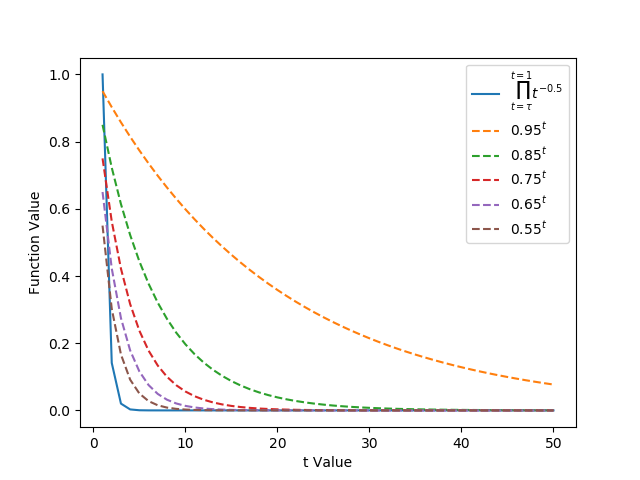
\includegraphics[width=\columnwidth]{decays}
  \vskip -0.06in
  \caption{Decay Functions Comparisons}
  \label{fig:decay}
\end{figure}

Figure \ref{fig:decay} shows that our power-law decay function decays much faster than the original exponential decay function. 
We believe that because new information is stored in a greater portion than before, the fast weights has to decay its existing memory quicker to prevent memory interference. 
This design also forces the RNN to learn patterns quicker from the fast weights since existing information is quickly removed.

\section{Experiments and Results}
We evaluate three RNN models on the associative retrieval tasks on three difficulty levels.
Our data consists of sequences of key-value pairs concatenated with two question marks and one query key.
The keys are lower case characters from the English alphabet chosen randomly without replacement, and the values are digits among 0 to 9 chosen randomly with replacement.

Our training data contains $100,000$ sequences and our testing data contains $50,000$ sequences.
The difficulty levels are three key-value pairs (K = $3$), four key-value pairs (K = $4$), and twenty-six key-value pairs (K = $26$).
The following models are evaluated on correctly predicting the associated value of the query key: a vanilla RNN (CONTROL), the original fast weights model (RNN-LN-FW), and the improved fast weights model (RNN-LN-FW2).
%RNN with LN (RNN-LN), GRU with LN (GRU-LN), RNN with LN and the original fast weights (RNN-LN-FW), RNN with LN and the improved fast weights (RNN-LN-FW2), RNN with the original fast weights (RNN-FW), and RNN with the improved fast weights (RNN-FW2).

\begin{table}[h!]
\centering
\vskip -0.12in
\caption{Testing Accuracy of Different Models}
\vskip 0.12in
\resizebox{!}{!}{
\begin{tabular}{cccc}
Model & \makecell{K = $3$} & \makecell{K = $4$} & \makecell{K = $26$} \\
\midrule
RNN-LN-FW2 & {$\bf 99.74\%$} & {$\bf 100\%$} & {$\bf 100\%$} \\
\midrule
RNN-LN-FW & $99.5\%$ & $99.71\%$ & $94.75\%$ \\
\midrule
\makecell{CONTROL} & $42.71\%$ & $34.49\%$ & $12.07\%$\\
\end{tabular}}
\label{table:compare_methods}
\end{table}

\begin{figure}[h]
\vskip -0.30in
  \centering
  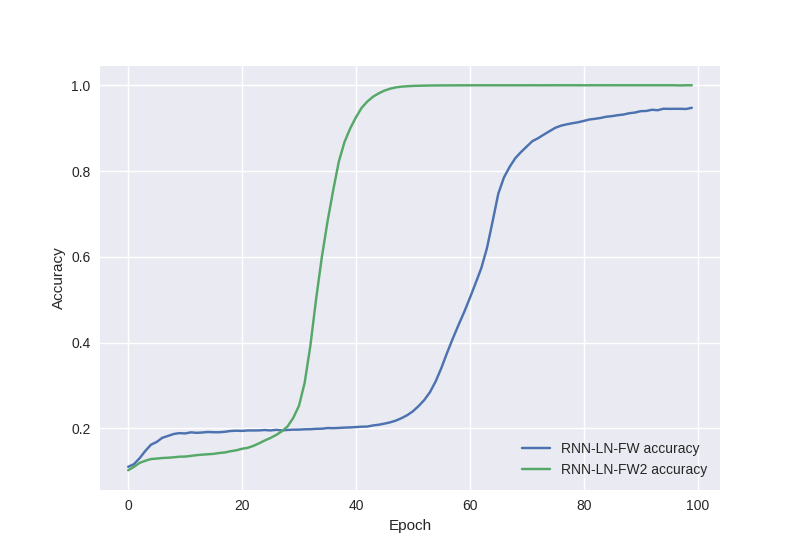
\includegraphics[width=\columnwidth]{k26}
  \vskip -0.06in
  \caption{Testing Accuracy K = 26}
  \label{fig:tea}
\end{figure}

Table \ref{table:compare_methods} and Figure \ref{fig:tea} show that our method leads to a faster convergence and a stronger testing accuracy for the fast Weights model. 

%\begin{figure}[h]
%  \centering
%  \includegraphics[width=\columnwidth]{training_accuracy}
%  \caption{Training Accuracy}
%  \label{fig:tra}
%\end{figure}

%\begin{figure}[h]
%  \centering
%  \includegraphics[width=\columnwidth]{training_loss}
%  \caption{Training Loss}
%  \label{fig:trl}
%\end{figure}

%\begin{figure}[h]
%  \centering
%  \includegraphics[width=\columnwidth]{testing_loss}
%  \caption{Testing Loss}
%  \label{fig:tel}
%\end{figure}


\section{Conclusion}
We introduce an enhanced fast weights model by incorporating memory consolidation designs from \cite{pld}.
We show that our model works better on the associative retrieval tasks and converges faster.
Our next direction is to evaluate the models on more difficult tasks such as sorting and repeated-copying.


\bibliographystyle{apacite}

\setlength{\bibleftmargin}{.125in}
\setlength{\bibindent}{-\bibleftmargin}

\bibliography{ccn_style}


\end{document}
